% Options for packages loaded elsewhere
\PassOptionsToPackage{unicode}{hyperref}
\PassOptionsToPackage{hyphens}{url}
\PassOptionsToPackage{dvipsnames,svgnames*,x11names*}{xcolor}
%
\documentclass[
  10pt,
  ignorenonframetext,
  aspectratio=43,
]{beamer}
\usepackage{pgfpages}
\setbeamertemplate{caption}[numbered]
\setbeamertemplate{caption label separator}{: }
\setbeamercolor{caption name}{fg=normal text.fg}
\beamertemplatenavigationsymbolsempty

%%
%%% Definition of colors
%%% Source: https://latexcolor.com/
\definecolor{blanchedalmond}{rgb}{1.0, 0.92, 0.8}
\definecolor{blond}{rgb}{0.98, 0.94, 0.75}
%%% End of definition of colors
%%

% Prevent slide breaks in the middle of a paragraph
\widowpenalties 1 10000
\raggedbottom
\usepackage{lmodern}
\usepackage{amssymb,amsmath}
\usepackage{ifxetex,ifluatex}
\ifnum 0\ifxetex 1\fi\ifluatex 1\fi=0 % if pdftex
  \usepackage[T1]{fontenc}
  \usepackage[utf8]{inputenc}
  \usepackage{textcomp} % provide euro and other symbols
\else % if luatex or xetex
  \usepackage{unicode-math}
  \defaultfontfeatures{Scale=MatchLowercase}
  \defaultfontfeatures[\rmfamily]{Ligatures=TeX,Scale=1}
  \setmainfont[]{Myriad Pro}
  \ifxetex
    \usepackage{xeCJK}
    \setCJKmainfont[ItalicFont=AR PL UKai TW]{AR UDJingXiHeiPU30}
  \fi
  \ifluatex
    \usepackage[]{luatexja-fontspec}
    \setmainjfont[ItalicFont=AR PL UKai TW]{AR UDJingXiHeiPU30}
  \fi
\fi
\usetheme[]{metropolis}
\usecolortheme{metropolis}
\usefonttheme{serif} % use mainfont rather than sansfont for slide text
% Use upquote if available, for straight quotes in verbatim environments
\IfFileExists{upquote.sty}{\usepackage{upquote}}{}
\IfFileExists{microtype.sty}{% use microtype if available
  \usepackage[]{microtype}
  \UseMicrotypeSet[protrusion]{basicmath} % disable protrusion for tt fonts
}{}
\makeatletter
\@ifundefined{KOMAClassName}{% if non-KOMA class
  \IfFileExists{parskip.sty}{%
    \usepackage{parskip}
  }{% else
    \setlength{\parindent}{0pt}
    \setlength{\parskip}{6pt plus 2pt minus 1pt}}
}{% if KOMA class
  \KOMAoptions{parskip=half}}
\makeatother
\usepackage{xcolor}
\IfFileExists{xurl.sty}{\usepackage{xurl}}{} % add URL line breaks if available
\IfFileExists{bookmark.sty}{\usepackage{bookmark}}{\usepackage{hyperref}}
\hypersetup{
  pdftitle={Social Media and Fake News in the 2016 Election},
  pdfauthor={Yu-Hsin Ho},
  colorlinks=true,
  linkcolor=Maroon,
  filecolor=Maroon,
  citecolor=Blue,
  urlcolor=red,
  pdfcreator={LaTeX via pandoc}}
\urlstyle{same} % disable monospaced font for URLs
\newif\ifbibliography
\usepackage{listings}
\newcommand{\passthrough}[1]{#1}
\lstset{defaultdialect=sh}
\lstset{framexleftmargin=0mm, frame=trBL,backgroundcolor=\color{blanchedalmond!5},numbers=left,numberstyle=\scriptsize,basicstyle=\small}
\lstset{aboveskip=5mm,belowskip=5mm,xleftmargin=20pt,xrightmargin=5pt}
% \lstset{prebreak={\raisebox{0ex}[0ex][0ex]}}
% \lstset{postbreak={\raisebox{0ex}[0ex][0ex]\space}}
\lstset{breaklines=true,breakatwhitespace=true}
\usepackage{longtable,booktabs}
\usepackage{graphicx,grffile}
\makeatletter
\def\maxwidth{\ifdim\Gin@nat@width>\linewidth\linewidth\else\Gin@nat@width\fi}
\def\maxheight{\ifdim\Gin@nat@height>\textheight\textheight\else\Gin@nat@height\fi}
\makeatother
% Scale images if necessary, so that they will not overflow the page
% margins by default, and it is still possible to overwrite the defaults
% using explicit options in \includegraphics[width, height, ...]{}
\setkeys{Gin}{width=\maxwidth,height=\maxheight,keepaspectratio}
% Set default figure placement to htbp
\makeatletter
\def\fps@figure{htbp}
\makeatother
\setlength{\emergencystretch}{3em} % prevent overfull lines
\providecommand{\tightlist}{%
  \setlength{\itemsep}{0pt}\setlength{\parskip}{0pt}}
\setcounter{secnumdepth}{-\maxdimen} % remove section numbering

%
% When using babel or polyglossia with biblatex, loading csquotes is recommended 
% to ensure that quoted texts are typeset according to the rules of your main language.
%
\usepackage{csquotes}

%
% blockquote
%
\definecolor{blockquote-border}{RGB}{221,221,221}
\definecolor{blockquote-text}{RGB}{89,89,89}
\usepackage{mdframed}
\newmdenv[rightline=false,bottomline=false,topline=false,linewidth=3pt,linecolor=blockquote-border,skipabove=\parskip]{customblockquote}
\renewenvironment{quote}{\begin{customblockquote}\list{}{\rightmargin=0em\leftmargin=0em}%
\item\relax\color{blockquote-text}\ignorespaces}{\unskip\unskip\endlist\end{customblockquote}}

%
% Source Sans Pro as the de­fault font fam­ily
% Source Code Pro for monospace text
%
% 'default' option sets the default 
% font family to Source Sans Pro, not \sfdefault.
%

\usepackage{adjustbox}
\usepackage{booktabs}
\linespread{1.3}
\setlength{\parskip}{1em}

\title{Social Media and Fake News in the 2016 Election}
\subtitle{Allcott, H., \& Gentzkow, M. (2017). Journal of Economic
Perspectives. doi:10.1257/jep.31.2.211}
\author{Yu-Hsin Ho}
\date{March 22, 2022}
\institute{Department of Economics, National Taiwan University}

\begin{document}
\frame{\titlepage}

\begin{frame}
  \tableofcontents[hideallsubsections]
\end{frame}
\hypertarget{motivation}{%
\section{Motivation}\label{motivation}}

\begin{frame}{Motivation}
Why Social Media? Why Fake News?

\begin{itemize}
\tightlist
\item
  62\% adult American use social media to consume news
\item
  Fake news are mostly circulated through social media
\item
  Social media had lowered the entry barrier of news market, potentially
  brought more low quality sources into the market.
\item
  Most popular fake news inclined to favor Donald Trump, which might
  affect the result of 2016 presidential election.
\end{itemize}
\end{frame}

\begin{frame}
\begin{figure}
\centering
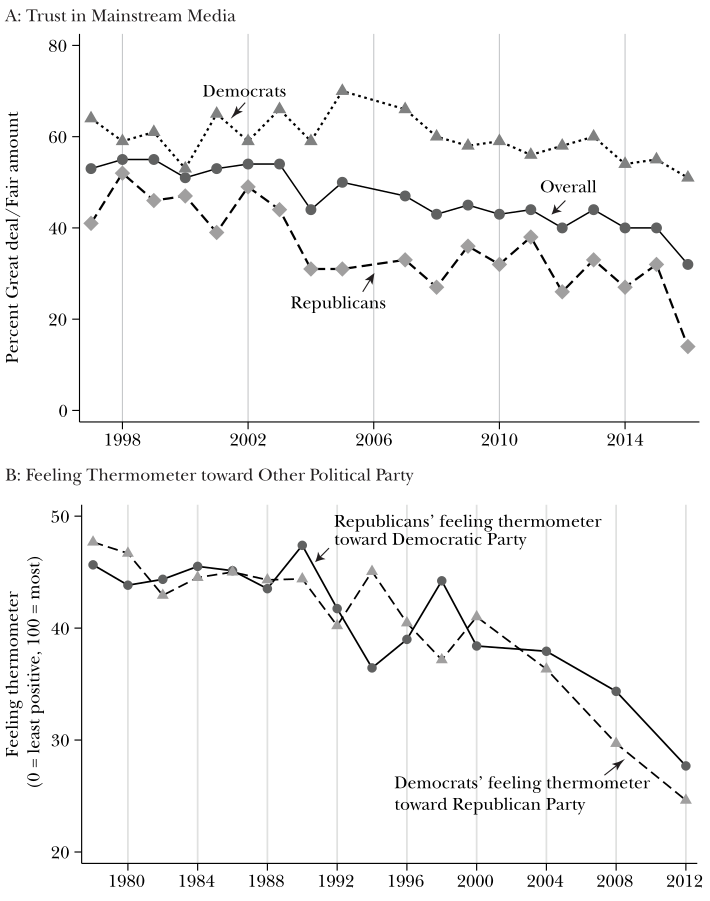
\includegraphics[width=0.6\textwidth,height=\textheight]{20220315-allcott-gentzkow-2016-election-fake-news.assets/image-20220314191028856.png}
\caption{Trends Related to Fake News}
\end{figure}
\end{frame}

\begin{frame}{Definition of Fake News}
\protect\hypertarget{definition-of-fake-news}{}
News articles that are \textbf{intentionally} and \textbf{verifiably
false}, and could mislead readers.

Not including: conspiracy theories that aren't falsifiable.
\end{frame}

\hypertarget{a-model-of-news-market}{%
\section{A Model of News Market}\label{a-model-of-news-market}}

\begin{frame}{A Model of News Market}
\begin{figure}
\centering
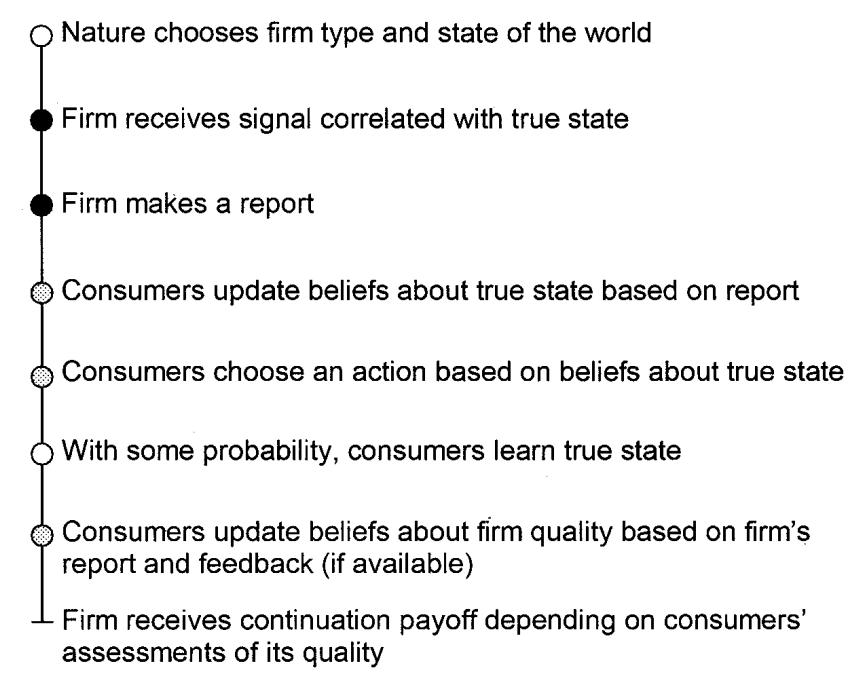
\includegraphics[width=0.8\textwidth,height=\textheight]{20220315-allcott-gentzkow-2016-election-fake-news.assets/image-20220314191927957.png}
\caption{Timing of the monopoly game (Gentzkow \& Shapiro, 2006)}
\end{figure}
\end{frame}

\begin{frame}{Supply Side}
\protect\hypertarget{supply-side}{}
\begin{enumerate}
\tightlist
\item
  There are 2 \textbf{unobserved} state of the world: Clinton or Trump
  will perform better in office.
\item
  Firms obtained signals correlated with true state through journalism.
\item
  Each firms owned a \textbf{report strategy} that mapped the signal
  into their publication: Report truthfully or biased.
\end{enumerate}
\end{frame}

\begin{frame}{Demand Side}
\protect\hypertarget{demand-side}{}
\begin{enumerate}
\tightlist
\item
  Consumers have their own (heterogeneous) prior beliefs on the true
  state of the world.
\item
  Consumers' utility come from (1) learning truth, and (2) confirming
  their prior beliefs.

  \begin{enumerate}
  \tightlist
  \item
    Specifically, they must ``vote the right person''
  \item
    \textbf{Trade-off}: legitimate news v.s. false news but which made
    them happy
  \end{enumerate}
\end{enumerate}
\end{frame}

\begin{frame}{Feedback}
\protect\hypertarget{feedback}{}
\begin{itemize}
\tightlist
\item
  Consumers update their belief on quality of media firms through their
  posterior observation on the true state of the world.

  \begin{itemize}
  \tightlist
  \item
    E.g. Observing the performance of Donald Trump while he's in office.
  \end{itemize}
\item
  Consumers choose whether to consume in future periods.
\item
  Media firms have incentives to enlarge their audience base due to
  advertising revenue.
\end{itemize}
\end{frame}

\begin{frame}{Incentives to Produce Fake News}
\protect\hypertarget{incentives-to-produce-fake-news}{}
\begin{enumerate}
\tightlist
\item
  Feedback is limited/expensive, rational consumers tends to judge fake
  news outlet to be higher quality, inflecting future consumption.
\item
  Fake news that confirms prior beliefs might increase consumers'
  utility.
\end{enumerate}

Model implication: Fake news is like media bias, which is mostly induced
by consumer's preference.
\end{frame}

\begin{frame}{Implications on Fake News}
\protect\hypertarget{implications-on-fake-news}{}
Characteristics of fake news producers:

\begin{enumerate}
\tightlist
\item
  No investment in journalism. (zero correlation between their signal
  and true state)
\item
  Do not attempt to build long-term reputation.
\end{enumerate}

Reasons why consumers would buy it:

\begin{enumerate}
\tightlist
\item
  Hard to observe the true state
\item
  News confirming beliefs increase private utility
\end{enumerate}
\end{frame}

\begin{frame}
\begin{block}{Externalities and Welfare Loss}
\protect\hypertarget{externalities-and-welfare-loss}{}
\begin{enumerate}
\tightlist
\item
  Inaccurate signals decrease the private utility provided by knowing
  the truth.
\item
  False beliefs might undermine democratic process.
\item
  Consumers might be more skeptical towards legitimate news.
\item
  Fake news reduce the incentive of high-quality media to invest in
  journalism.
\end{enumerate}
\end{block}
\end{frame}

\hypertarget{real-data-on-fake-news}{%
\section{Real Data on Fake News}\label{real-data-on-fake-news}}

\begin{frame}{Real Data on Fake News}
\begin{itemize}
\tightlist
\item
  Fake news headlines: gathered from fact check websites/columns

  \begin{itemize}
  \tightlist
  \item
    Snopes.com: 138 articles
  \item
    PolitiFact.com: 13 articles
  \item
    BuzzFeed: 21 articles
  \end{itemize}
\item
  Facebook share data: BuzzSumo
\item
  Website traffic data: Alexa
\end{itemize}
\end{frame}

\begin{frame}
\begin{figure}
\centering
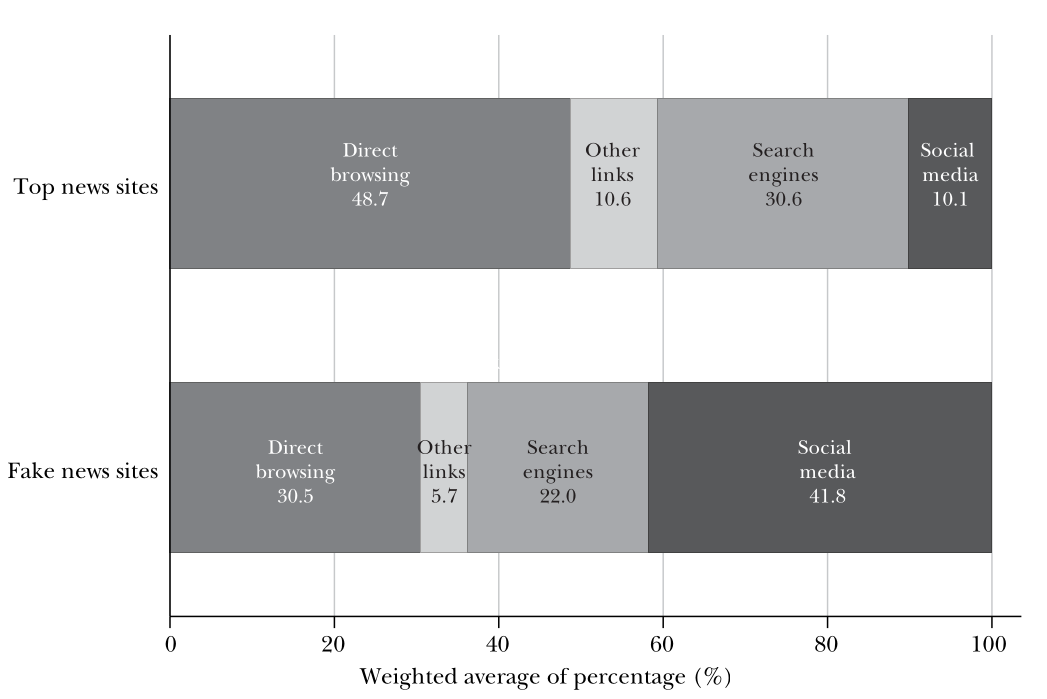
\includegraphics{20220315-allcott-gentzkow-2016-election-fake-news.assets/image-20220314203702283.png}
\caption{Share of Visits to US News Websites by Source}
\end{figure}
\end{frame}

\begin{frame}
\begin{block}{Partisanship}
\protect\hypertarget{partisanship}{}
Among 156 fake news articles:

\begin{itemize}
\tightlist
\item
  41 pro-Clinton, 115 pro-Trump
\item
  7.6 million and 30.3 million times shared respectively
\end{itemize}
\end{block}
\end{frame}

\hypertarget{exposure-to-fake-news}{%
\section{Exposure to Fake News}\label{exposure-to-fake-news}}

\begin{frame}{Post-Election Survey}
\protect\hypertarget{post-election-survey}{}
\begin{itemize}
\tightlist
\item
  November 28, 2016 (3 weeks after election)
\item
  Sample: 1208 US adults
\item
  Online questionaire
\item
  Questions

  \begin{itemize}
  \tightlist
  \item
    How much time spent on election news, and by how much through social
    media?
  \item
    What's your most important news source?
  \end{itemize}
\item
  15 headlines selected randomly out of 30

  \begin{itemize}
  \tightlist
  \item
    Have you seen this headline?
  \item
    Do you think it's true?
  \item
    Some were placebo headlines to detect false recall.
  \end{itemize}
\item
  Reweighted to fit nationwide demographic characteristics
\end{itemize}
\end{frame}

\begin{frame}
\begin{figure}
\centering
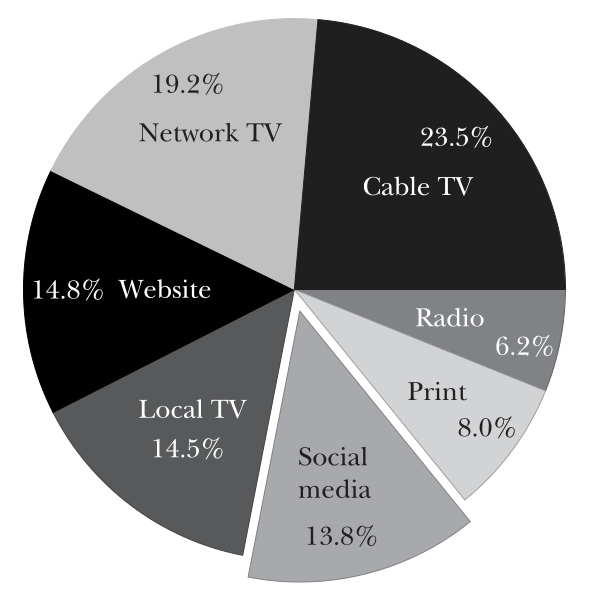
\includegraphics[width=0.7\textwidth,height=\textheight]{20220315-allcott-gentzkow-2016-election-fake-news.assets/image-20220314204054746.png}
\caption{Most Important Source of 2016 Election News}
\end{figure}
\end{frame}

\begin{frame}
\begin{figure}
\centering
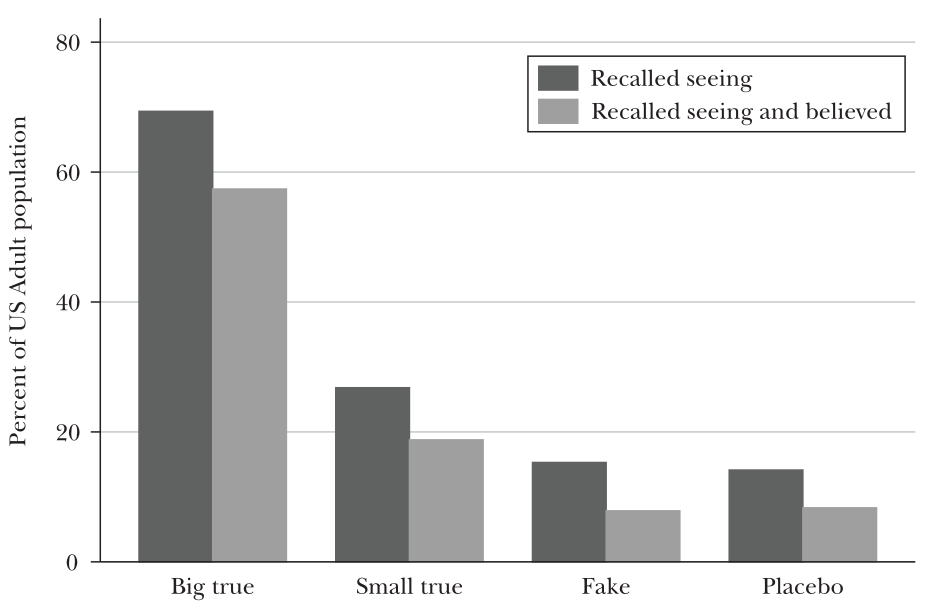
\includegraphics[width=0.7\textwidth,height=\textheight]{20220315-allcott-gentzkow-2016-election-fake-news.assets/image-20220314204225668.png}
\caption{Percent of US Adult Population that Recall Seeing or that
Believed Election News}
\end{figure}

\center{Fake - Placebo = 1.2\%}
\end{frame}

\begin{frame}
\begin{block}{Imputing Exposure of Fake News}
\protect\hypertarget{imputing-exposure-of-fake-news}{}
\begin{itemize}
\tightlist
\item
  Average share per article = 0.386 million
\item
  Recalled seeing = 1.2\%
\item
  Chance of recalled exposure = 1.2\% / 0.386 = 3\% (per million shares)
\item
  3\% \(\times\) 38 million (Total shares) = 1.14 (per adult)
\end{itemize}
\end{block}
\end{frame}

\hypertarget{who-believes-fake-news}{%
\section{Who Believes Fake News}\label{who-believes-fake-news}}

\begin{frame}{Who's Outperforming in Distinguishing Fake News?}
\protect\hypertarget{whos-outperforming-in-distinguishing-fake-news}{}
\[
C_{i a} = \alpha_{1} \mathbf{X}_{i}+\alpha_{0}+\varepsilon_{i a}
\]

for respondent \(i\), headline \(a\).

Outcome \(C_{i a} = 1\) if correctly identify the truthfulness of
headline, 0.5 if respondent is not sure, 0 otherwise.

Dependent variable \(\mathbf{X}_i\) is a vector of individual
characteristics
\end{frame}

\begin{frame}
\begin{figure}
\centering
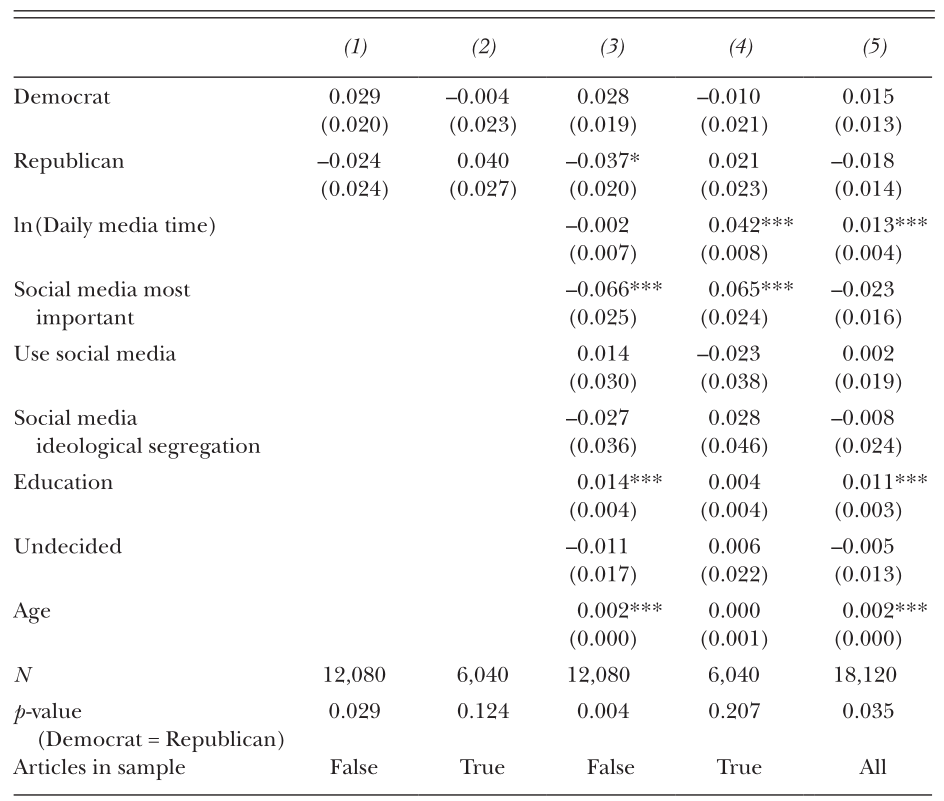
\includegraphics[width=0.75\textwidth,height=\textheight]{20220315-allcott-gentzkow-2016-election-fake-news.assets/image-20220314152113796.png}
\caption{What Predicts Correct Beliefs about News Headlines?}
\end{figure}
\end{frame}

\begin{frame}{Ideological Alignment and Belief of News Headlines}
\protect\hypertarget{ideological-alignment-and-belief-of-news-headlines}{}
\[
B_{i a}=\beta_{D} D_{i} C_{a}+\beta_{R} R_{i} T_{a}+\gamma_{D} D_{i}+\gamma_{R} R_{i}+\varepsilon_{i a}
\]

for respondent \(i\), headline \(a\)

\(B_{i a}\) = 1 for believing the article is real, 0.5 if not sure, 0 if
no.

\(D_i\) for self-reported Democrat, \(C_a\) for pro-Clinton headline.

\(R_i\) for self-reported Republican, \(T_a\) for pro-Trump headline.

Headlines are assigned randomly and equally with true/false,
pro-Clinton/pro-Trump.

\begin{itemize}
\tightlist
\item
  \(\beta\) captures the aligned ideology effect
\item
  \(\gamma\) captures partisanship effect
\end{itemize}
\end{frame}

\begin{frame}
\begin{figure}
\centering
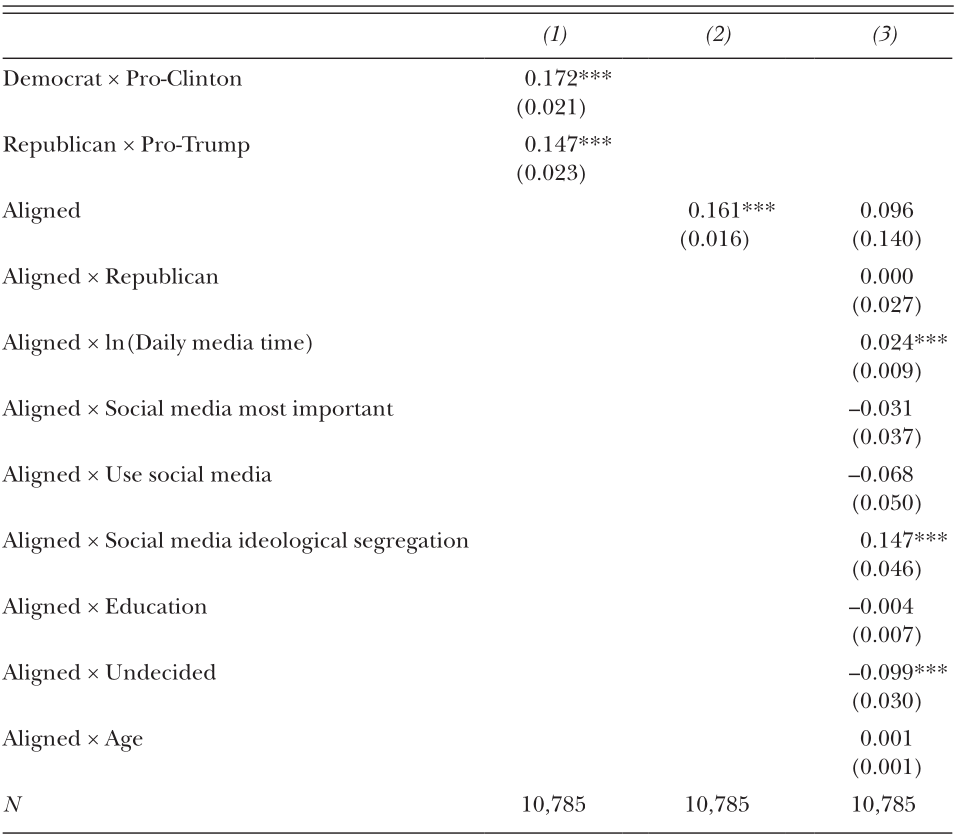
\includegraphics[width=0.7\textwidth,height=\textheight]{20220315-allcott-gentzkow-2016-election-fake-news.assets/image-20220314182649354.png}
\caption{Ideological Alignment and Belief of News Headlines}
\end{figure}

\emph{Differences between Democrats and Republicans in the magnitude of
ideologically aligned inference are not statistically significant.}
\end{frame}

\hypertarget{contribution}{%
\section{Contribution}\label{contribution}}

\begin{frame}{Contribution}
\begin{quote}
We do not provide an assessment of this claim (fake news pivoting
election result) one way or another.
\end{quote}

\begin{itemize}
\tightlist
\item
  An descriptive overview of fake news exposure during 2016 U.S.
  presidential election.
\item
  Media literacy, instead of partisanship, better explains the ability
  to distinguish fake news.
\item
  Both Democrats and Republicans tends to believe in the
  ideologically-aligned news.
\end{itemize}
\end{frame}

\end{document}
